\section{\large \textcolor{blue}{Relatividade restrita}}

\begin{flushleft}
\textbf{\textcolor{blue}{\Large Quest\~ao 51}}\\
\noindent
\subsection{Quest\~ao 51 - Lei de Stefan--Boltzmann}
Se a temperatura de um corpo negro dobra, a potência total
irradiada por unidade de área

\begin{itemize}
\item[(A)] aumenta por um fator 2.
\item[(B)] aumenta por um fator 4.
\item[(C)] aumenta por um fator 8.
\item[(D)] aumenta por um fator 16.
\end{itemize}

\vspace{0.5cm}

\textcolor{red}{\textbf{Solução:}}\\
\section*{Variação da potência irradiada por um corpo negro ao dobrar a temperatura}

De acordo com a \textbf{lei de Stefan--Boltzmann}, a potência irradiada por unidade de área \( P/A \) de um corpo negro é dada por:
\[
\frac{P}{A} = \sigma T^4,
\]
onde:
\begin{itemize}
    \item \( \sigma \approx 5,67 \times 10^{-8} \, \text{W/m}^2\cdot\text{K}^4 \) é a constante de Stefan--Boltzmann;
    \item \( T \) é a temperatura absoluta do corpo em kelvins.
\end{itemize}

Suponha que a temperatura inicial do corpo seja \( T_0 \), e a potência inicial irradiada por unidade de área seja:
\[
\left( \frac{P}{A} \right)_0 = \sigma T_0^4.
\]

Quando a temperatura dobra (\( T = 2T_0 \)), a nova potência irradiada por unidade de área é:
\[
\frac{P}{A} = \sigma (2T_0)^4 = \sigma \cdot 2^4 T_0^4 = 16 \cdot \sigma T_0^4.
\]

Ou seja:
\[
\frac{P}{A} = 16 \cdot \left( \frac{P}{A} \right)_0
\]

\section*{Resposta final}

Se a temperatura de um corpo negro dobra, a potência irradiada por unidade de área aumenta 16 vezes.

A resposta correta é alternativa \colorbox{green!50}{\textbf{D}}.
\end{flushleft}

\noindent\rule{\linewidth}{0.6pt}\\

\section*{Aplicação da Lei do Deslocamento de Wien}

A \textbf{Lei do Deslocamento de Wien} estabelece uma relação inversa entre o comprimento de onda no qual a emissão de radiação de um corpo negro é máxima e a sua temperatura absoluta. Matematicamente:
\[
\lambda_{\text{pico}} \cdot T = b
\]

onde:
\begin{itemize}
    \item \( \lambda_{\text{pico}} \) é o comprimento de onda de pico (em metros),
    \item \( T \) é a temperatura absoluta (em kelvins),
    \item \( b = 2,897 \times 10^{-3} \, \mathrm{m \cdot K} \) é a constante de Wien.
\end{itemize}

\subsection*{Importância e aplicações}

A Lei de Wien é amplamente utilizada para:
\begin{itemize}
    \item Determinar a temperatura de estrelas, planetas e outros corpos celestes a partir de suas curvas espectrais.
    \item Estimar a cor de um corpo aquecido (por exemplo, metais incandescentes em fundições).
    \item Diagnóstico em processos industriais de aquecimento, fornos e lâmpadas.
    \item Prever a emissão dominante de radiação térmica em diferentes temperaturas.
\end{itemize}

\subsection*{Exemplos práticos}

\begin{enumerate}
    \item \textbf{O Sol:}  
    O pico de emissão do Sol está em aproximadamente \( \lambda_{\text{pico}} = 500\,\mathrm{nm} \) (luz verde). Aplicando a Lei de Wien:
    \[
    T = \frac{b}{\lambda_{\text{pico}}} = \frac{2,897 \times 10^{-3}}{500 \times 10^{-9}} \approx 5794\,\mathrm{K}.
    \]
    Portanto, a temperatura superficial do Sol é cerca de \( 5800\,\mathrm{K} \).

    \item \textbf{Uma lâmpada incandescente:}  
    Para uma lâmpada cujo filamento brilha com pico em \( \lambda_{\text{pico}} = 1000\,\mathrm{nm} \) (infravermelho próximo):
    \[
    T = \frac{2,897 \times 10^{-3}}{1000 \times 10^{-9}} \approx 2897\,\mathrm{K}.
    \]
    Essa é uma temperatura típica do filamento de tungstênio.

    \item \textbf{Uma estrela fria:}  
    Uma estrela com temperatura superficial \( T = 3000\,\mathrm{K} \) emite radiação de pico em:
    \[
    \lambda_{\text{pico}} = \frac{b}{T} = \frac{2,897 \times 10^{-3}}{3000} \approx 966\,\mathrm{nm}.
    \]
    O que está no infravermelho próximo.
\end{enumerate}

\subsection*{Resumo}

A Lei de Wien é uma ferramenta fundamental para relacionar a cor aparente ou o comprimento de onda dominante da radiação emitida por 
um corpo negro à sua temperatura, permitindo medições indiretas de temperatura em muitas áreas da ciência e tecnologia.

\begin{flushleft}
\textbf{\textcolor{blue}{\Large Quest\~ao 52}}\\
\noindent
Observe o gráfico a seguir.

\begin{figure}[h]
\centering
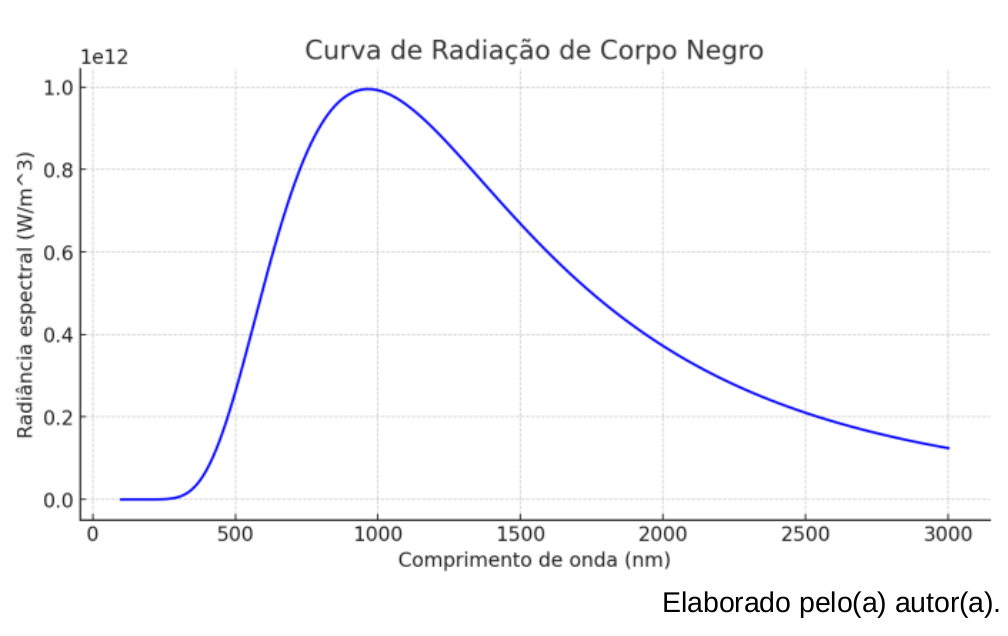
\includegraphics[scale=0.5]{figures/radiacaocorponegro.png}
\end{figure}
\subsection{Quest\~ao 52 - Temperatura de um corpo negro usando a lei de Wien}
O gráfico acima mostra a curva de radiância espectral de um
corpo negro, com o pico da emissão ocorrendo em 966 nm.
Utilizando a Lei de Wien, que relaciona o comprimento de
onda de pico da emissão de um corpo negro com a sua
temperatura, selecione a resposta que mais se aproxima do
resultado calculado para a temperatura desse corpo negro.
(Dados: Constante de deslocamento de Wien $b = 2{,}897 \times 10^{-3}\,\mathrm{m}\,.\mathrm{K}.)$

\begin{itemize}
\item[(A)] 3000 K.
\item[(B)] 3100 K.
\item[(C)] 3300 K.
\item[(D)] 3900 K.
\end{itemize}

\vspace{0.5cm}

\textcolor{red}{\textbf{Solução:}}\\

\section*{Determinação da temperatura de um corpo negro usando a lei de Wien}

A \textbf{lei do deslocamento de Wien} estabelece que:
\[
\lambda_{\text{pico}} \cdot T = b
\]

onde:
\begin{itemize}
    \item \( \lambda_{\text{pico}} \) é o comprimento de onda no qual a radiância espectral é máxima (em metros),
    \item \( T \) é a temperatura absoluta do corpo negro (em kelvins),
    \item \( b = 2,897 \times 10^{-3} \, \mathrm{m\cdot K} \) é a constante de deslocamento de Wien.
\end{itemize}

\section*{Dados do problema:}

O pico da emissão ocorre em:
\[
\lambda_{\text{pico}} = 966 \, \mathrm{nm} = 966 \times 10^{-9} \, \mathrm{m} = 9,66 \times 10^{-7} \, \mathrm{m}.
\]

\section*{Cálculo da temperatura:}

A temperatura é dada por:
\[
T = \frac{b}{\lambda_{\text{pico}}}
\]

Substituindo os valores:
\[
T = \frac{2,897 \times 10^{-3}}{9,66 \times 10^{-7}}.
\]

Efetuando a divisão:
\[
T \approx 2998 \, \mathrm{K}.
\]

\section*{Resposta final:}

\[
\boxed{
T \approx 3000 \, \mathrm{K}
}
\]

Portanto, a temperatura do corpo negro é aproximadamente \( \mathbf{3000\,K} \).

A resposta correta é alternativa \colorbox{green!50}{\textbf{A}}.
\end{flushleft}

\noindent\rule{\linewidth}{0.6pt}\\

\begin{flushleft}
\textbf{\textcolor{blue}{\Large Quest\~ao 53}}\\
\noindent
\subsection{Quest\~ao 53 - Efeito fotoelétrico}
Uma superfície metálica é exposta a luz de comprimento de onda de 400 nm para induzir o efeito fotoelétrico. A função
trabalho do metal é de 2,0 eV. São dadas a Constante de Planck $h = 6{,}626 \times 10^{-34} J.s$, a velocidade da luz 
$c = 3{,}0 \times 10^8 m/s$ e $e = 1{,}602 \times 10^{-19} J$. Utilizando a equação do efeito fotoelétrico podemos 
determinar a energia cinética máxima dos elétrons ejetados da superfície metálica, que

\begin{itemize}
\item[(A)] 0,95 eV.
\item[(B)] 1,10 eV.
\item[(C)] 1,25 eV.
\item[(D)] 1,50 eV.
\end{itemize}

\vspace{0.5cm}

\textcolor{red}{\textbf{Solução:}}\\

\section*{Efeito Fotoelétrico: Cálculo da energia cinética máxima}

Uma superfície metálica é iluminada com luz de comprimento de onda \( \lambda = 400\,\mathrm{nm} \), e sua função trabalho é:
\[
W_0 = 2{,}0\,\mathrm{eV}.
\]

Queremos calcular a energia cinética máxima \( K_{\text{máx}} \) dos elétrons ejetados.

\section*{Equação do efeito fotoelétrico}

A equação do efeito fotoelétrico é:
\[
E_f = W_0 + K_{\text{máx}},
\]
onde \(E_f\) é a energia do fóton incidente:
\[
E_f = h\nu = \frac{hc}{\lambda}.
\]

\section*{Conversão de unidades}

O comprimento de onda em metros:
\[
\lambda = 400\,\mathrm{nm} = 400 \times 10^{-9}\,\mathrm{m}.
\]

A constante de Planck:
\[
h = 6{,}626 \times 10^{-34}\, \mathrm{J\cdot s}.
\]

Velocidade da luz:
\[
c = 3{,}0 \times 10^{8}\, \mathrm{m/s}.
\]

\section*{Energia do fóton}

Calculamos \(E_f\) em joules:
\[
E_f = \frac{hc}{\lambda} =
\frac{6{,}626 \times 10^{-34} \cdot 3{,}0 \times 10^{8}}{400 \times 10^{-9}}.
\]

Efetuando a conta:
\[
E_f \approx 4{,}97 \times 10^{-19}\, \mathrm{J}.
\]

Convertendo para elétron-volts (\(1\,\mathrm{eV} = 1{,}602 \times 10^{-19}\,\mathrm{J}\)):
\[
E_f = \frac{4{,}97 \times 10^{-19}}{1{,}602 \times 10^{-19}} \approx 3,1\,\mathrm{eV}.
\]

\section*{Energia cinética máxima}

Usamos:
\[
K_{\text{máx}} = E_f - W_0.
\]

Substituindo os valores:
\[
K_{\text{máx}} = 3{,}1\,\mathrm{eV} - 2{,}0\,\mathrm{eV} = 1{,}1\,\mathrm{eV}.
\]

\section*{Resposta final}

\[
\boxed{
K_{\text{máx}} \approx 1{,}1\,\mathrm{eV}
}
\]

A energia cinética máxima dos elétrons ejetados é aproximadamente \(1{,}1\,\mathrm{eV}\).

A resposta correta é alternativa \colorbox{green!50}{\textbf{B}}.
\end{flushleft}

\noindent\rule{\linewidth}{0.6pt}\\

\begin{flushleft}
\textbf{\textcolor{blue}{\Large Quest\~ao 54}}\\
\noindent
\subsection{Quest\~ao 54 - Efeito fotoelétrico}
No efeito fotoelétrico ocorre a emissão de elétrons de uma
superfície metálica quando radiação incide sobre essa
superfície. A radiação mais eficaz para que o efeito
fotoelétrico ocorra é a

\begin{itemize}
\item[(A)] radiação de raios X.
\item[(B)] radiação infravermelha.
\item[(C)] radiação ultravioleta.
\item[(D)] radiação de micro-ondas.
\end{itemize}

\vspace{0.5cm}

\textcolor{red}{\textbf{Solução:}}\\

\section*{Efeito Fotoelétrico: Resolução e valores típicos da função trabalho}

Quando luz incide sobre a superfície de um metal, elétrons podem ser ejetados se a energia do fóton \( E_f \) for maior ou igual à função trabalho \( W_0 \) do metal:
\[
E_f = W_0 + K_{\text{máx}}
\]

onde:
\begin{itemize}
    \item \( E_f = \frac{hc}{\lambda} \) é a energia do fóton;
    \item \( W_0 \) é a função trabalho do metal;
    \item \( K_{\text{máx}} \) é a energia cinética máxima dos elétrons.
\end{itemize}

\section*{Resolução do problema:}

\textbf{Dados:}
\[
\lambda = 400\,\mathrm{nm}, \quad W_0 = 2{,}0\,\mathrm{eV}, \quad hc = 1240\,\mathrm{eV\cdot nm}.
\]

Energia do fóton:
\[
E_f = \frac{1240}{400} = 3{,}1\,\mathrm{eV}.
\]

Energia cinética máxima:
\[
K_{\text{máx}} = E_f - W_0 = 3{,}1 - 2{,}0 = 1{,}1\,\mathrm{eV}.
\]

\textbf{Resposta:}
\[
\boxed{
K_{\text{máx}} \approx 1{,}1\,\mathrm{eV}
}
\]

\section*{Função trabalho de alguns metais e comprimentos de onda limites:}

A função trabalho \( W_0 \) está relacionada ao comprimento de onda máximo \( \lambda_{\text{lim}} \) para que o efeito fotoelétrico ocorra:
\[
\lambda_{\text{lim}} = \frac{hc}{W_0}
\]

com \( hc = 1240\,\mathrm{eV\cdot nm} \).

\bigskip

\begin{center}
\renewcommand{\arraystretch}{1.3}
\begin{tabular}{|c|c|c|}
\hline
\textbf{Metal} & \textbf{Função trabalho \( W_0~(\mathrm{eV}) \)} & \textbf{\( \lambda_{\text{lim}}~(\mathrm{nm}) \)} \\
\hline
Césio (Cs)     & 1,9 & 653 \\ \hline
Potássio (K)   & 2,3 & 539 \\ \hline
Sódio (Na)     & 2,7 & 459 \\ \hline
Cálcio (Ca)    & 3,2 & 388 \\ \hline
Cobre (Cu)     & 4,7 & 264 \\ \hline
Prata (Ag)     & 4,3 & 288 \\ \hline
Ouro (Au)      & 5,1 & 243 \\ \hline
\hline
\end{tabular}
\end{center}

\section*{Resumo:}
\begin{itemize}
    \item A energia cinética máxima dos elétrons ejetados é a diferença entre a energia do fóton incidente e a função trabalho.
    \item Quanto menor a função trabalho, maior o comprimento de onda limite para o efeito fotoelétrico.
    \item Metais alcalinos (como césio e potássio) são mais fáceis de ionizar.
\end{itemize}

A resposta correta é alternativa \colorbox{green!50}{\textbf{C}}.
\end{flushleft}

\noindent\rule{\linewidth}{0.6pt}\\

\begin{flushleft}
\textbf{\textcolor{blue}{\Large Quest\~ao 55}}\\
\noindent
\subsection{Quest\~ao 55 - Efeito Compton}
Um fóton com um comprimento de onda inicial de \(0,10\,\text{nm}\) colide com um elétron inicialmente em repouso.  
Após a colisão, o fóton é espalhado com um ângulo de \(60^\circ\) em relação à sua direção original.  
Sabendo que \(\cos 60^\circ = 0,5\), dada a constante de Compton \(2,43 \times 10^{-12}\,m\) e usando a fórmula do 
efeito Compton para calcular a mudança no comprimento de onda do fóton espalhado, podemos determinar o novo comprimento 
de onda do fóton após o espalhamento, que é de:


\begin{itemize}
\item[(A)] 0{,}102 nm.
\item[(B)] 0{,}222 nm.
\item[(C)] 0{,}220 nm.
\item[(D)] 0{,}232 nm.
\end{itemize}

\vspace{0.5cm}

\textcolor{red}{\textbf{Solução:}}\\

\section*{Efeito Compton: Cálculo do novo comprimento de onda do fóton}

Um fóton com comprimento de onda inicial:
\[
\lambda_0 = 0{,}10\,\mathrm{nm} = 1{,}0 \times 10^{-10}\,\mathrm{m}
\]

é espalhado por um elétron inicialmente em repouso, formando um ângulo de:
\[
\theta = 60^\circ.
\]

Sabemos que:
\[
\cos 60^\circ = 0{,}5
\]

e a \textbf{constante de Compton} do elétron é:
\[
\lambda_C = 2{,}43 \times 10^{-12}\,\mathrm{m}.
\]

\section*{Fórmula do efeito Compton}

A variação no comprimento de onda do fóton é dada por:
\[
\Delta \lambda = \lambda_C (1 - \cos\theta)
\]

Substituindo os valores:
\[
\Delta \lambda =
2{,}43 \times 10^{-12} \cdot (1 - 0{,}5) =
2{,}43 \times 10^{-12} \cdot 0{,}5 =
1{,}215 \times 10^{-12}\,\mathrm{m}.
\]

\section*{Novo comprimento de onda}

O novo comprimento de onda do fóton é:
\[
\lambda = \lambda_0 + \Delta\lambda
\]

Substituindo:
\[
\lambda =
1{,}0 \times 10^{-10} + 1{,}215 \times 10^{-12} =
1{,}01215 \times 10^{-10}\,\mathrm{m}.
\]

Convertendo para nanômetros (\(1\,\mathrm{nm} = 10^{-9}\,\mathrm{m}\)):
\[
\lambda =
0{,}101215\,\mathrm{nm}.
\]

\section*{Resposta final}

\[
\boxed{
\lambda \approx 0{,}1012\,\mathrm{nm}
}
\]

O novo comprimento de onda do fóton espalhado é aproximadamente \(0{,}1012\,\mathrm{nm}\).

A resposta correta é alternativa \colorbox{green!50}{\textbf{A}}.
\end{flushleft}

\noindent\rule{\linewidth}{0.6pt}\\

\begin{flushleft}
\textbf{\textcolor{blue}{\Large Quest\~ao 56}}\\
\noindent
\subsection{Quest\~ao 56 - Efeito Compton}
No efeito Compton, um fóton incide sobre um elétron inicialmente em repouso e é espalhado, fazendo com que o elétron recue.  
Quando o ângulo de espalhamento \( \varphi \) varia de \(0^\circ\) a \(90^\circ\), o ângulo de recuo do elétron \( \theta \) 
varia no intervalo:


\begin{itemize}
\item[(A)] $0^{\circ} \leq \theta \leq 180^{\circ}$.
\item[(B)] $0^{\circ} \leq \theta < 90^{\circ}$.
\item[(C)] $0^{\circ} \leq \theta < 120^{\circ}$.
\item[(D)] $90^{\circ} \leq \theta < 120^{\circ}$.
\end{itemize}

\vspace{0.5cm}

\textcolor{red}{\textbf{Solução:}}\\

\section*{Demonstração da relação entre os ângulos no efeito Compton}

No efeito Compton, um fóton incide com momento \( \vec{p}_\gamma \) e energia \( E_\gamma = h\nu \) sobre um elétron em repouso.  
Após a colisão:
\begin{itemize}
    \item o fóton é espalhado com ângulo \( \varphi \) e comprimento de onda aumentado (\( \lambda' \)),
    \item o elétron recua com ângulo \( \theta \) e energia cinética \( K \).
\end{itemize}

\subsection*{Conservação da quantidade de movimento}

No sistema de coordenadas onde o fóton inicial se propaga ao longo do eixo \(x\), temos:
\[
\vec{p}_\gamma = p_\gamma \hat{x}
\]

e após a colisão:
\[
\vec{p}_\gamma' = p_\gamma' \bigl( \cos\varphi\,\hat{x} + \sin\varphi\,\hat{y} \bigr)
\]
\[
\vec{p}_e = p_e \bigl( \cos\theta\,\hat{x} + \sin\theta\,\hat{y} \bigr)
\]

\subsection*{Componentes no eixo \(x\)}

\[
p_\gamma = p_\gamma' \cos\varphi + p_e \cos\theta
\]

\subsection*{Componentes no eixo \(y\)}

\[
0 = p_\gamma' \sin\varphi - p_e \sin\theta
\]

Da segunda equação, obtemos:
\[
p_e \sin\theta = p_\gamma' \sin\varphi
\]

Da primeira equação, isolamos \( p_e \cos\theta \):
\[
p_e \cos\theta = p_\gamma - p_\gamma' \cos\varphi
\]

\subsection*{Tangente do ângulo \( \theta \)}

Dividindo as componentes \(y/x\), temos:
\[
\tan\theta = \frac{p_e \sin\theta}{p_e \cos\theta} =
\frac{p_\gamma' \sin\varphi}{p_\gamma - p_\gamma' \cos\varphi}
\]

\subsection*{Expressando em termos de energias}

Sabemos que \( p_\gamma = \frac{E_\gamma}{c} \) e \( p_\gamma' = \frac{E_\gamma'}{c} \), onde \( E_\gamma' \) é a energia do fóton espalhado:
\[
E_\gamma' = \frac{E_\gamma}{1 + \frac{E_\gamma}{m_e c^2}(1 - \cos\varphi)}
\]

Substituímos \( p_\gamma' \) na equação anterior para obter \( \tan\theta \) em função de \( \varphi \) e \( E_\gamma \).

\section*{Resultado final:}

A relação geral é:
\[
\tan\theta =
\frac{\sin\varphi}{\displaystyle \frac{E_\gamma}{E_\gamma'} - \cos\varphi}
\]

ou ainda, substituindo \( E_\gamma' \):
\[
\tan\theta =
\frac{\sin\varphi}{\displaystyle \left( 1 + \frac{E_\gamma}{m_e c^2}(1 - \cos\varphi) \right) - \cos\varphi}
\]

Essa é a relação entre o ângulo de espalhamento do fóton \( \varphi \) e o ângulo de recuo do elétron \( \theta \) no efeito Compton.

O \(E_\gamma\) é a energia inicial do fóton, e definimos a razão adimensional:

\[
\alpha =
\frac{E_\gamma}{m_e c^2}.
\]

Substituindo \(\alpha\), a expressão fica:

\[
\tan\theta =
\frac{\sin\varphi}{
\big(1 + \alpha(1-\cos\varphi)\big) - \cos\varphi}.
\]

\section*{Limite quando \(\varphi \to 0^\circ\)}

Para \(\varphi \to 0^\circ\), temos:
\[
\sin\varphi \to 0, \quad \cos\varphi \to 1.
\]

No denominador:
\[
\big(1 + \alpha(1-\cos\varphi)\big) - \cos\varphi 
\to (1 + 0) - 1 = 0.
\]

Portanto:
\[
\tan\theta \to 0 \quad \implies \quad \theta \to 0.
\]

\section*{Limite quando \(\varphi = 90^\circ\)}

Para \(\varphi = 90^\circ\), temos:
\[
\sin\varphi = 1, \quad \cos\varphi = 0.
\]

No denominador:
\[
\big(1 + \alpha(1-0)\big) - 0 =
1 + \alpha.
\]

Logo:
\[
\tan\theta =
\frac{1}{1+\alpha}.
\]

Observações:
\begin{itemize}
    \item Para fótons de baixa energia (\(\alpha \ll 1\)): \(1+\alpha \approx1\), então \(\tan\theta\approx1\), ou seja, \(\theta\approx45^\circ\).
    \item Para fótons de alta energia (\(\alpha\gg1\)): \(1+\alpha\) é grande, então \(\tan\theta\approx0\), ou seja, \(\theta\) pequeno.
\end{itemize}

Portanto, mesmo para \(\varphi=90^\circ\), o ângulo \(\theta\) permanece \textbf{menor que \(90^\circ\)}.

\section*{Conclusão}

O ângulo de recuo do elétron \(\theta\) varia no intervalo:
\[
\boxed{0^\circ \leq \theta < 90^\circ}
\]


A resposta correta é alternativa \colorbox{green!50}{\textbf{B}}.
\end{flushleft}

\noindent\rule{\linewidth}{0.6pt}\\

\begin{flushleft}
\textbf{\textcolor{blue}{\Large Quest\~ao 57}}\\
\noindent
\subsection{Quest\~ao 57 - Energia total relativística do elétron}
Sabendo que a massa do elétron é \( 9,11 \times 10^{-31}\, \mathrm{kg} \), a velocidade da luz é 
\( 3 \times 10^8\, \mathrm{m/s} \) e \( 1\,\mathrm{eV} = 1{,}602 \times 10^{-19}\, \mathrm{J} \), 
a energia total de um elétron movendo-se com uma velocidade de \( \left( \frac{\sqrt{3}}{2} \right) c \) é de:

\begin{itemize}
\item[(A)] $0{,}510$ MeV.
\item[(B)] $0{,}723$ MeV.
\item[(C)] $1{,}024$ MeV.
\item[(D)] $1{,}105$ MeV.
\end{itemize}

\vspace{0.5cm}

\textcolor{red}{\textbf{Solução:}}\\

\section*{Cálculo da energia total relativística do elétron}

\textbf{Dados:}
\begin{itemize}
    \item Massa do elétron: \(m_e = 9{,}11 \times 10^{-31}\, \mathrm{kg}\)
    \item Velocidade da luz: \(c = 3{,}0 \times 10^8\, \mathrm{m/s}\)
    \item \(1\,\mathrm{eV} = 1{,}602 \times 10^{-19}\, \mathrm{J}\)
    \item Velocidade do elétron: \(v = \frac{\sqrt{3}}{2} c\)
\end{itemize}

\subsection*{Fator de Lorentz}

A energia total relativística do elétron é dada por:
\[
E = \gamma m_e c^2
\]

com o fator de Lorentz:
\[
\gamma = \frac{1}{\sqrt{1 - \frac{v^2}{c^2}}}
\]

Sabemos que:
\[
\frac{v}{c} = \frac{\sqrt{3}}{2} \quad \implies \quad \left( \frac{v}{c} \right)^2 = \frac{3}{4}
\]

Portanto:
\[
\gamma = \frac{1}{\sqrt{1 - \frac{3}{4}}} =
\frac{1}{\sqrt{\frac{1}{4}}} =
2
\]

\subsection*{Energia de repouso do elétron}

A energia de repouso do elétron é:
\[
E_0 = m_e c^2
\]

Substituindo os valores:
\[
E_0 =
\left( 9{,}11 \times 10^{-31} \right) \cdot
\left( 3{,}0 \times 10^8 \right)^2 =
9{,}11 \times 10^{-31} \cdot 9{,}0 \times 10^{16} =
8{,}199 \times 10^{-14}\, \mathrm{J}
\]

\subsection*{Energia total do elétron}

\[
E = \gamma E_0 =
2 \cdot 8{,}199 \times 10^{-14} =
1{,}6398 \times 10^{-13}\, \mathrm{J}
\]

\subsection*{Conversão para eV}

Sabemos que \(1\,\mathrm{eV} = 1{,}602 \times 10^{-19}\, \mathrm{J}\), então:
\[
E =
\frac{1{,}6398 \times 10^{-13}}{1{,}602 \times 10^{-19}} \approx
1{,}024 \times 10^6\, \mathrm{eV} =
1{,}024\,\mathrm{MeV}
\]

\subsection*{Resposta final:}

\[
\boxed{
E \approx 1{,}02\, \mathrm{MeV}
}
\]

\textbf{A energia total do elétron em movimento com velocidade \( \frac{\sqrt{3}}{2}c \) é aproximadamente: \(1{,}02\,\mathrm{MeV}\).}

A resposta correta é alternativa \colorbox{green!50}{\textbf{C}}.
\end{flushleft}

\noindent\rule{\linewidth}{0.6pt}\\

\begin{flushleft}
\textbf{\textcolor{blue}{\Large Quest\~ao 58}}\\
\noindent
\subsection{Quest\~ao 58 - Relatividade de uma nave espacial}
Uma nave espacial viaja a uma velocidade de \(0{,}85c\) em relação à Terra, sendo \(c = 3 \times 10^8\, \mathrm{m/s}\) 
a velocidade da luz no vácuo. Um relógio a bordo da nave marca 1 hora. Aproximando \( \sqrt{0{,}2775} = 0{,}53 \), 
durante esse tempo a distância percorrida e o tempo decorrido para um observador na Terra são, respectivamente:


\begin{itemize}
\item[(A)] Distância: \(1{,}7 \times 10^9\, km\), Tempo: \(1{,}9\) horas.
\item[(B)] Distância: \(1{,}7 \times 10^9\, km\), Tempo: \(3{,}8\) horas.
\item[(C)] Distância: \(3{,}1 \times 10^8\, km\), Tempo: \(2{,}9\) horas.
\item[(D)] Distância: \(3{,}1 \times 10^8\, km\), Tempo: \(3{,}9\) horas.
\end{itemize}

\vspace{0.5cm}

\textcolor{red}{\textbf{Solução:}}\\

\section*{Problema: nave viajando a \(0{,}85c\)}

Uma nave espacial viaja a uma velocidade \(v = 0{,}85c\), com \(c = 3{,}0 \times 10^8\, \mathrm{m/s}\).  
O relógio a bordo da nave marca um tempo próprio \(t_0 = 1\,\mathrm{h}\).  
Sabendo que \(\sqrt{0{,}2775} = 0{,}53\), queremos calcular:

\begin{itemize}
    \item A distância percorrida para um observador na Terra.
    \item O tempo decorrido para um observador na Terra.
\end{itemize}

\subsection*{Fator de Lorentz}

O tempo medido na Terra é dilatado:
\[
t = \gamma t_0
\]

com:
\[
\gamma = \frac{1}{\sqrt{1-\frac{v^2}{c^2}}}
\]

Calculamos:
\[
\left( \frac{v}{c} \right) = 0{,}85 \quad \implies \quad \left( \frac{v}{c} \right)^2 = 0{,}7225
\]

Logo:
\[
1 - \frac{v^2}{c^2} = 1 - 0{,}7225 = 0{,}2775
\]

Como \(\sqrt{0{,}2775} = 0{,}53\), temos:
\[
\gamma = \frac{1}{0{,}53} \approx 1{,}89
\]

Assim:
\[
t = \gamma t_0 = 1{,}89 \cdot 1 = 1{,}89\,\mathrm{h} \approx 1{,}9\,\mathrm{h}
\]

\subsection*{Distância percorrida na Terra}

Na Terra, a distância percorrida é:
\[
d = v t
\]

com:
\[
v = 0{,}85 \cdot 3{,}0 \times 10^8 = 2{,}55 \times 10^8\, \mathrm{m/s}
\]

Convertendo \(t = 1{,}9\,\mathrm{h}\) para segundos:
\[
t = 1{,}9 \cdot 3600 = 6840\,\mathrm{s}
\]

Então:
\[
d = 2{,}55 \times 10^8 \cdot 6840 \approx 1{,}744 \times 10^{12}\,\mathrm{m} = 1{,}744 \times 10^9\,\mathrm{km} \approx 1{,}7 \times 10^9\,\mathrm{km}
\]

\subsection*{Resposta final:}

\[
\boxed{
\text{Distância: } 1{,}7 \times 10^9\,\mathrm{km} \quad \text{Tempo: } 1{,}9\,\mathrm{h}
}
\]


A resposta correta é alternativa \colorbox{green!50}{\textbf{A}}.
\end{flushleft}

\noindent\rule{\linewidth}{0.6pt}\\


\begin{flushleft}
\textbf{\textcolor{blue}{\Large Quest\~ao 59}}\\
\noindent
\subsection{Quest\~ao 59 - Radioatividade}
Um hospital utiliza o isótopo radioativo Tecnécio-99m (\(^{99m}\mathrm{Tc}\)) para exames de diagnóstico por imagem.  
O Tecnécio-99m tem uma meia-vida de aproximadamente \(6\) horas. Se uma dose inicial de \(120\,\mathrm{mg}\) de Tecnécio-99m é 
administrada a um paciente, quanto tempo será necessário para que a quantidade de isótopo no corpo do paciente caia para \(15\,\mathrm{mg}\)?
(Dados: \(\ln 2 = 0{,}693\) e \(\ln(0{,}125) = -2{,}079\).)

\begin{itemize}
\item[(A)] 10 horas.
\item[(B)] 12 horas.
\item[(C)] 14 horas.
\item[(D)] 18 horas.
\end{itemize}

\vspace{0.5cm}

\textcolor{red}{\textbf{Solução:}}\\

\text{Dados:}

\begin{itemize}
    \item Meia-vida do Tecnécio-99m: \( T_{1/2} = 6 \) horas
    \item Dose inicial: \( N_0 = 120\,\mathrm{mg} \)
    \item Dose final desejada: \( N = 15\,\mathrm{mg} \)
    \item \(\ln 2 = 0{,}693\)
    \item \(\ln(0{,}125) = -2{,}079\)
\end{itemize}

\vspace{0.3cm}

\text{A quantidade de isótopo após um tempo \(t\) é dada por:}

\[
N = N_0 e^{-\lambda t}
\]

\text{onde \(\lambda\) é a constante de decaimento.}

\vspace{0.3cm}

\text{A constante \(\lambda\) está relacionada à meia-vida por:}

\[
T_{1/2} = \frac{\ln 2}{\lambda} \implies \lambda = \frac{\ln 2}{T_{1/2}} = \frac{0{,}693}{6} = 0{,}1155\,\mathrm{h}^{-1}
\]

\vspace{0.3cm}

\text{Queremos o tempo \(t\) para que a quantidade caia para \(15\,\mathrm{mg}\), ou seja:}

\[
\frac{N}{N_0} = e^{-\lambda t} \implies \ln\left(\frac{N}{N_0}\right) = -\lambda t \implies t = -\frac{1}{\lambda} \ln\left(\frac{N}{N_0}\right)
\]

\vspace{0.3cm}

\text{Calculando:}

\[
\frac{N}{N_0} = \frac{15}{120} = 0{,}125
\]

\[
t = -\frac{1}{0{,}1155} \ln(0{,}125) = -\frac{1}{0{,}1155} \times (-2{,}079) = \frac{2{,}079}{0{,}1155} \approx 18 \text{ horas}
\]

\vspace{0.3cm}

\boxed{
\text{Resposta: } t \approx 18 \text{ horas}}

A resposta correta é alternativa \colorbox{green!50}{\textbf{D}}.
\end{flushleft}

\noindent\rule{\linewidth}{0.6pt}\\

\begin{flushleft}
\textbf{\textcolor{blue}{\Large Quest\~ao 60}}\\
\noindent
\subsection{Quest\~ao 60 - Radioatividade}
Durante uma escavação arqueológica, um arqueólogo encontra restos de uma antiga fogueira contendo pedaços de madeira.  
A atividade do carbono-14 na amostra de madeira é medida e encontrada como sendo \(12{,}5\%\) da atividade do carbono-14 em organismos vivos.  
Sabendo que a meia-vida do carbono-14 é de aproximadamente \(5730\) anos, a idade da amostra de madeira pode ser determinada e vale:  
(Dados: \(\ln 2 = 0{,}693\) e \(\ln(0{,}125) = -2{,}079\).)

\begin{itemize}
\item[(A)] 5.730 anos.
\item[(B)] 8.585 anos.
\item[(C)] 11.460 anos.
\item[(D)] 17.190 anos.
\end{itemize}

\vspace{0.5cm}

\textcolor{red}{\textbf{Solução:}}\\

\text{Dados:}

\begin{itemize}
    \item Fração da atividade atual em relação à original: \(\frac{N}{N_0} = 12{,}5\% = 0{,}125\)
    \item Meia-vida do carbono-14: \(T_{1/2} = 5730 \text{ anos}\)
    \item \(\ln 2 = 0{,}693\)
    \item \(\ln(0{,}125) = -2{,}079\)
\end{itemize}

\vspace{0.3cm}

\text{A atividade após um tempo \(t\) é dada por:}

\[
N = N_0 e^{-\lambda t}
\]

\text{onde \(\lambda\) é a constante de decaimento.}

\vspace{0.3cm}

\text{Calculando \(\lambda\):}

\[
\lambda = \frac{\ln 2}{T_{1/2}} = \frac{0{,}693}{5730} \approx 1{,}21 \times 10^{-4}\, \text{ano}^{-1}
\]

\vspace{0.3cm}

\text{Determinando o tempo \(t\):}

\[
\frac{N}{N_0} = e^{-\lambda t} \implies \ln\left(\frac{N}{N_0}\right) = -\lambda t \implies t = -\frac{1}{\lambda} \ln\left(\frac{N}{N_0}\right)
\]

\vspace{0.3cm}

\text{Substituindo os valores:}

\[
t = -\frac{1}{1{,}21 \times 10^{-4}} \times \ln(0{,}125) = \frac{2{,}079}{1{,}21 \times 10^{-4}} \approx 17\,190 \text{ anos}
\]

\vspace{0.3cm}

\boxed{
\text{Resposta: } t \approx 17\,190 \text{ anos}
}

A resposta correta é alternativa \colorbox{green!50}{\textbf{D}}.
\end{flushleft}


\begin{flushleft}
\textbf{\textcolor{blue}{\Large Quest\~ao - IFFAR 2023 - Exploração Espacial e Relatividade}}\\
\noindent

\subsection{Quest\~ao - IFFAR 2023 - Exploração Espacial e Relatividade}

A Nasa (agência espacial dos EUA) anunciou, no início deste ano, a descoberta de um planeta com tamanho parecido com o da Terra 
e que pode ser habitável. Chamado de TOI 700, o planeta orbita a estrela anã TOI 700, em uma zona em que é possível haver água em 
estado líquido, crucial para a existência de vida como conhecemos. A estrela anã TOI 700 está localizada na constelação austral de 
Dorado, a 100 anos-luz de distância da Terra.

Embora a distância até o sistema TOI 700 seja impraticável de ser percorrida com a tecnologia atual, em filmes de ficção científica 
é comum a ideia de utilizar a dobra espacial para encurtar o tempo e a distância das viagens espaciais. Considerando um cenário 
hipotético no qual uma espaçonave pudesse realizar o percurso em um intervalo de tempo de 20 anos contados a partir do referencial 
da espaçonave, podemos explorar a ideia da dobra espacial. Nesse contexto fictício, a dobra espacial permitiria encurtar o espaço-tempo 
e criar um "atalho" entre dois pontos distantes no espaço. Dada essa premissa, qual seria, aproximadamente, a velocidade necessária para 
a nave conseguir realizar essa proeza?

\begin{itemize}
\item[(A)] $1{,}00c$
\item[(B)] $0{,}99c$
\item[(C)] $0{,}98c$
\item[(D)] $0{,}95c$
\item[(E)] $0{,}90c$
\end{itemize}

\vspace{0.5cm}

\textcolor{red}{\textbf{Solu\c{c}\~ao:}}\\

Sabemos que a distância entre a Terra e o sistema TOI 700 é de $d = 100$ anos-luz e o tempo medido no referencial da espaçonave é 
$t' = 20$ anos. Como o tempo é medido no referencial da nave, devemos aplicar a dilatação do tempo da Relatividade Restrita:

\[
t' = \frac{t}{\gamma}
\]

Em que:

\[
\gamma = \frac{1}{\sqrt{1 - \left(\frac{v}{c}\right)^2}}
\quad \text{e} \quad
t = \frac{d}{v}
\]

Substituindo na fórmula:

\[
t' = \frac{d}{v \gamma}
\Rightarrow v\gamma = \frac{d}{t'} = \frac{100}{20} = 5
\]

Substituímos o fator de Lorentz:

\[
v \cdot \frac{1}{\sqrt{1 - \left( \frac{v}{c} \right)^2}} = 5
\]

Seja $x = \frac{v}{c}$, temos:

\[
\frac{x}{\sqrt{1 - x^2}} = 5
\Rightarrow x = 5 \sqrt{1 - x^2}
\]

Elevando ao quadrado:

\[
x^2 = 25(1 - x^2) \Rightarrow x^2 + 25x^2 = 25 \Rightarrow 26x^2 = 25 \Rightarrow x^2 = \frac{25}{26}
\]

\[
x = \sqrt{\frac{25}{26}} = \frac{5}{\sqrt{26}} \approx 0{,}980
\]

Portanto, a velocidade necessária é aproximadamente:

\[
\frac{v}{c} \approx 0{,}98c
\]

\vspace{0.2cm}

A resposta correta é a alternativa \colorbox{green!50}{\textbf{C)}}.

\end{flushleft}

\begin{flushleft}
\textbf{\textcolor{blue}{\Large Quest\~ao 36 - IFSC 2023 - Efeito Fotoelétrico}}\\
\noindent

\subsection{Quest\~ao 36 - IFSC 2023 - Efeito Fotoelétrico}
O efeito fotoelétrico é um fenômeno no qual a luz incidente em um material pode arrancar 
elétrons desse material. O estudo do efeito fotoelétrico por Albert Einstein, em 1905, foi 
fundamental para o desenvolvimento da teoria quântica da luz e lhe rendeu o Prêmio Nobel de Física em 1921.

\textbf{Análise das lacunas:}

\begin{enumerate}
    \item A energia dos fótons é dada por:
    \[
    E_f = h f
    \]
    ou seja, depende da \textbf{frequência} (\(f\)) da luz.  
    Para que ocorra a emissão de elétrons, essa energia deve ser maior que a \textbf{função trabalho} (\(W\)), que é a energia mínima necessária para retirar um elétron do material.

    \item A \textbf{quantidade} de fotoelétrons emitidos depende:
    \begin{itemize}
        \item da \textbf{intensidade} da luz incidente (mais fótons → mais elétrons emitidos),
        \item e da \textbf{superfície} do material (propriedades físicas afetam o número de elétrons que podem ser liberados).
    \end{itemize}

    \item O \textbf{local} de onde os elétrons são arrancados:
    \begin{itemize}
        \item Em metais: elétrons vêm da \textbf{superfície}.
        \item Em semicondutores: elétrons vêm da banda de \textbf{valência}.
    \end{itemize}
\end{enumerate}

\textbf{Preenchendo as lacunas:}

\[
\text{(frequência) - (função trabalho) - (intensidade) - (superfície) - (valência)}
\]

Isso corresponde à alternativa:

\[
\boxed{\text{A}}
\]

\end{flushleft}


\begin{flushleft}
\textbf{\textcolor{blue}{\Large Quest\~ao - }}\\
\noindent

\subsection{Quest\~ao }

\begin{itemize}
\item[(A)] 
\item[(B)] 
\item[(C)]
\item[(D)] 
\item[(E)] 
\end{itemize}

\vspace{0.5cm}

\textcolor{red}{\textbf{Solução:}}\\


A resposta correta é alternativa \colorbox{green!50}{\textbf{...}}.

\end{flushleft}